\subsection{Screen overlays}
At certain stages of the game, we need to display overlays, containing important information and/or buttons for navigation.
The game screen contains the four overlays; Starting, Paused, Crashed, and Won, which are described hereafter.
All of the overlays can be seen in \cref{sprint2:overlays:fig}.

\begin{figure}[h]
	\centering
    \begin{subfigure}[b]{0.49\textwidth}
            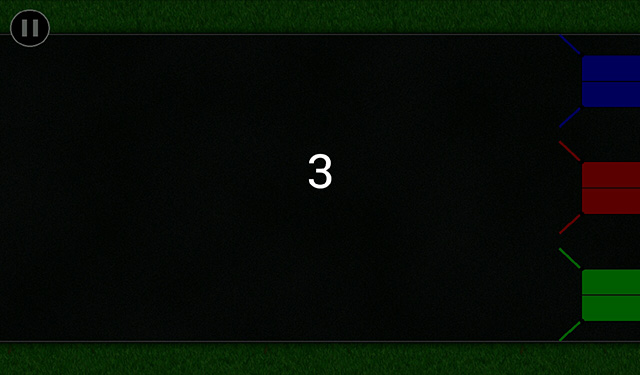
\includegraphics[width=\textwidth]{screen_starting}
            \caption{Starting overlay}
            \label{sprint2:overlays:fig:starting}
    \end{subfigure}
    \begin{subfigure}[b]{0.49\textwidth}
            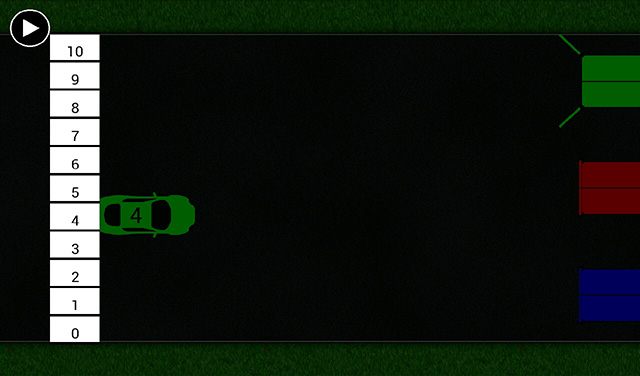
\includegraphics[width=\textwidth]{screen_paused}
            \caption{Paused overlay}
            \label{sprint2:overlays:fig:paused}
    \end{subfigure}
    \begin{subfigure}[b]{0.49\textwidth}
            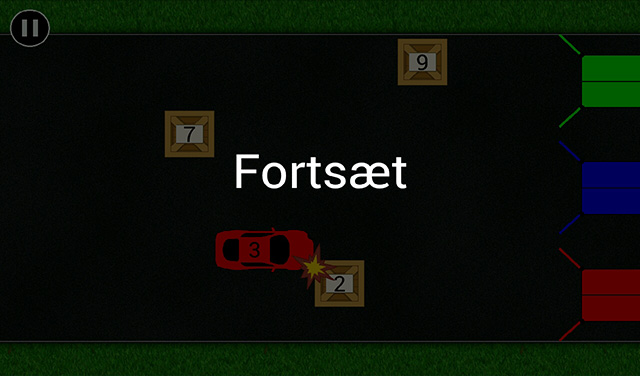
\includegraphics[width=\textwidth]{screen_crashed}
            \caption{Crash overlay}
            \label{sprint2:overlays:fig:crashed}
    \end{subfigure}
    \begin{subfigure}[b]{0.49\textwidth}
            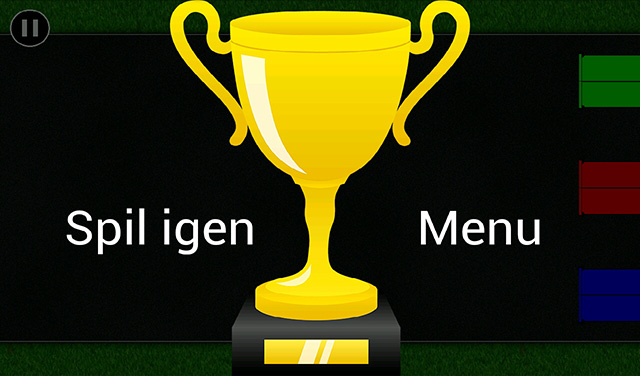
\includegraphics[width=\textwidth]{screen_won}
            \caption{Won overlay}
            \label{sprint2:overlays:fig:won}
    \end{subfigure}
    \caption{The four overlays for the game}
    \label{sprint2:overlays:fig}
\end{figure}

\paragraph{Starting Overlay} is displayed when a new game is started (from either the main menu or the Win Overlay).
It is a short countdown, enabling the player to get ready, as opposed to starting the game straight away, or simply waiting without any feedback for the player.
It is a 3 second countdown (3.. 2.. 1.. Go), as can be seen in \cref{sprint2:overlays:fig:starting}.

\paragraph{Paused overlay} is linked to requirement \ref{sprint2:requirements:pause}, which states: \textit{It should be possible to pause the game. When the game is paused, a loudness-barometer is displayed next to the car, further visualizing the current loudness.}
At all times when in the game screen, a pause button is visible in the top left corner.
When pressed, the game is paused (the car stops moving) and the loudness gauge is displayed (see \cref{sprint2:overlays:fig:paused}).

\paragraph{Crashed overlay} is for when the citizen hits an obstacle or a wrong garage.
It is a simple screen displaying an explosion at the impact spot, stopping the game and awaiting the 'Continue' button to be pressed.
The crash overlay can be seen in \cref{sprint2:overlays:fig:crashed}.

\paragraph{Won overlay} is displayed after all garages have been closed.
This is linked to requirement \ref{sprint2:requirements:reward}, which states: \textit{When the game is won a reward should be given}.
A trophy is displayed along with two buttons; 'Play again' and 'Menu'.
The overlay can be seen in \cref{sprint2:overlays:fig:won}.